\documentclass[12pt]{article}
\usepackage{tikz}
\usepackage{pgfplots}
\pgfplotsset{compat=1.13}

\usepackage{extsizes}
\usepackage{caption}
\usepackage{multirow}
\usepackage{wrapfig}

\renewcommand{\epsilon}{\ensuremath{\varepsilon}}
\renewcommand{\phi}{\ensuremath{\varphi}}
\renewcommand{\kappa}{\ensuremath{\varkappa}}
\renewcommand{\le}{\ensuremath{\leqslant}}
\renewcommand{\leq}{\ensuremath{\leqslant}}
\renewcommand{\ge}{\ensuremath{\geqslant}}
\renewcommand{\geq}{\ensuremath{\geqslant}}
\renewcommand{\emptyset}{\varnothing}

\newcommand{\lw}{\linewidth}
\usepackage{geometry} % Простой способ задавать поля
\geometry{top=30mm}
\geometry{bottom=30mm}
\geometry{left=25mm}
\geometry{right=20mm}

\usepackage[T2A]{fontenc}			% кодировка
\usepackage[utf8]{inputenc}	
\usepackage[english,russian]{babel}   %% загружает пакет многоязыковой вёрстки
\usepackage{indentfirst}
\usepackage{subfigure}
\usepackage{amsmath,amsfonts,amssymb,amsthm,mathtools} 
\usepackage{graphicx}

\usepackage{pdfpages}

\begin{document}
	\begin{minipage}{0.45\linewidth}
	Работу выполнили\\
	Самохин Валентин,\\
	Юрченко Петр\\ 676 гр.\\[2mm]
	под руководством\\
	Нухова А.\,К\,.
	\end{minipage}
	\hfill
	\begin{minipage}{0.45\linewidth}\flushright
		Маршрут~VIII \ №~5\\[3mm]
		27~марта 2018~г.,\\
		\end{minipage}
		
		\vspace{8mm}
		\begin{center}
			\textbf{\Large Лабораторная работа №~4.3.1:}\\[\parskip]
			\LARGE Изучение дифракции света
			\end{center}
			\vspace{0mm}
			\paragraph{Цель работы:}
				 исследовать явления дифракции Френеля и Фраунгофера на щели, изучить влияние дифракции на разрешающую способность оптических инструментов.
				

			
			\paragraph{В работе используются:}
			оптическая скамья, ртутная лампа, монохроматор, щели с регулируемой шириной, рамка с вертикальной нитью, двойная щель, микроскоп на поперечных салазках с микрометрическим винтом, зрительная труба.
			
			
			\vspace{2\parskip}
		\paragraph{Теоретическая справка.}
		Дифракцией, в самом широком смысле слова, называют отклонения
		в распространении волн от законов геометрической оптики. Частный
		случай дифракции - огибание волной препятствия и её проникновение
		в область геометрической тени.
		
		Основными параметрами, существенно определяющими характер дифракционных явлений, являются длина волны $\lambda$,
		размер отверстия $b$ и расстояние до плоскости наблюдения $z$. Как показывает дальнейший анализ, характер дифракционных явлений определяется значением волнового параметра
		$$\dfrac{\sqrt{\lambda z}}{b}.$$
		\begin{itemize}
			\item $p \ll 1$ : геометрическая оптика
			\item $p \gg 1$ : дифракция Фраунгофера
			\item $p \sim 1$ : дифракция Френеля
		\end{itemize}
	
		\paragraph{Примеры тонких экранов (транспарантов)}
		
		\begin{enumerate}
			\item Амплитудная синусоидальная решётка - тонкая пластинка, амплитудная прозрачность которой меняется от точки к точке по закону
			$$t(x) = \beta(1 + m\cos \Omega x),$$
			где $m=const$ - глубина модуляции, $\Omega = \frac{2\pi}{d}$ - пространственная частота решетки с периодом $d$.
			
			\item Дифракционная решетка - непрозрачный экран с рядом параллельных равноотстоящих щелей, $d$ -  период решётки, $b$ - ширина щелей.
			
			
			Если амплитудная прозрачность транспаранта не меняется от точки к точке, а изменяется только набег фазы $\phi(x, y)$, то такой транспарант называется фазовым. 
			\item Фазовая синусоидальная решетка
			$$t(x) = \exp^{im\cos\Omega x} \approx 1 + im\cos \Omega x$$
			
			\item Тонкая линза
			$$t(x, y) = \exp^{-i\frac{k}{2f}(x^2 + y^2)}$$
			
		\end{enumerate}
	
	\paragraph{Принцип Гюйгегнса - Френеля}
	
	Согласно принципу Гюйгенса, каждую точку,
	куда пришла волна, можно рассматривать как источник вторичной волны. То есть можно представить	себе, что волна возбуждает колебания некоторого фиктивного источника (осциллятора), который и переизлучает вторичную волну. Частота $\omega$
	этой переизлучённой волны совпадает с частотой исходной монохроматической волны. Френель дополнил принцип Гюйгенса, предложив
	рассматривать световое колебание в любой точке наблюдения в области
	$z > 0$ как результат интерференции этих вторичных волн.
	
	\paragraph{Дифракция Френеля}
	
	\subparagraph{На круглом отверстии.}При дифракции Френеля на круглом отверстии интенсивность в точке $P$, находящейся на оси отверстия на расстоянии $z$ от него, равна
	$$I = 2I_0(1-\cos(\dfrac{k}{2z}r^2)).$$
	
	Минимумы(четные) и максимумы(нечетные) достигаются при значения радиуса отверстия
	$$\boxed{r_m = \sqrt{m\lambda z}}$$
	
	 Пластинка, делающая синфазными вклады $dA$ от каждого ее участка, есть тонкая линза с фокусным расстоянием $f = z$.
	 
	\begin{center} 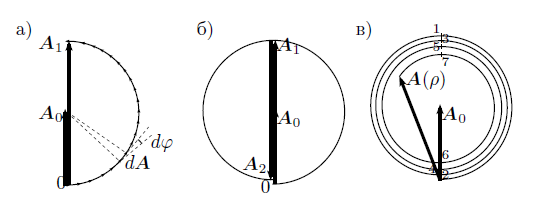
\includegraphics{amp_method}
	 \captionof{figure}{Метод векторных диаграмм}
	\end{center}
 
	 \subparagraph{Пятно Пуассона.}
	 Амплитуда в центре геометрической тени малого препятствия (шарика или диска) остаётся почти такой же, как если бы это препятствие отсутствовало.
	
	\subparagraph{На щели}
	
	В данном случае вместо кольцевых зон Френеля мы имеем зоны в виде полос (их называют
	зонами Шустера). Вклад от каждой следующей
	зоны Шустера в колебание в точке наблюдения находится в противофазе (разность фаз $\pi$)
	с вкладом от предыдущей зоны.
	
	
	Продолжая дальше построение векторной
	диаграммы, придём к спирали Корню.
	
	\begin{figure}
	
		\begin{minipage}[h]{0.49\linewidth}
			\centering{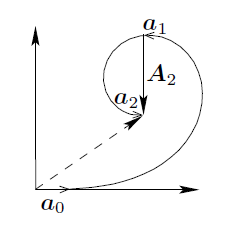
\includegraphics[width=0.5\linewidth]{Shuster2} \\ Две зоны Шустера}
			
		\end{minipage}
		\hfill
		\begin{minipage}[h]{0.49\linewidth}
			\centering{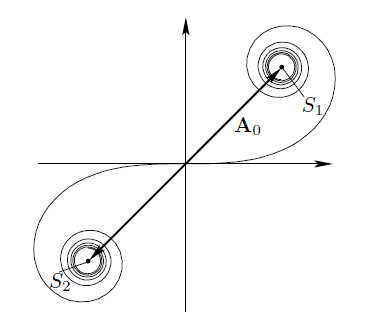
\includegraphics[width=0.5\linewidth]{kornu} \\ Спираль Корню}
		\end{minipage}
		
	\end{figure}
	
	$m$-я зона Шустера --- это полоса, внешний край которой отстоит от точки наблюдения на расстояние $z + m\lambda/2$ и на расстояние $\xi_m = \sqrt{m\lambda z}$.
	
	\paragraph{Дифракция Фраунгофера}
	\subparagraph{На щели.}
	$$g(\theta) \propto \dfrac{\sin (\frac{kb}{2}\sin \theta)}{\frac{kb}{2}\sin\theta}$$
	
	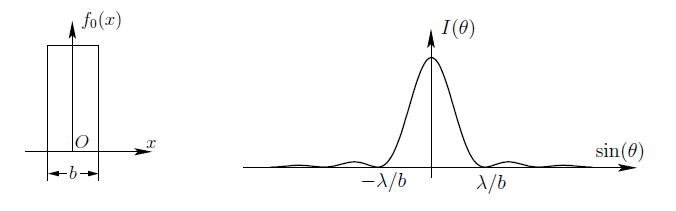
\includegraphics{fraun_one}
	\captionof{figure}{Поле и угловое распределение интенсивности при дифракции на щели}
	\subparagraph{На двух щелях.}
	$$I(\theta) = |g(\theta)^2|\cdot(1 + \cos(kd\sin \theta))^2$$
	\begin{center}
		
	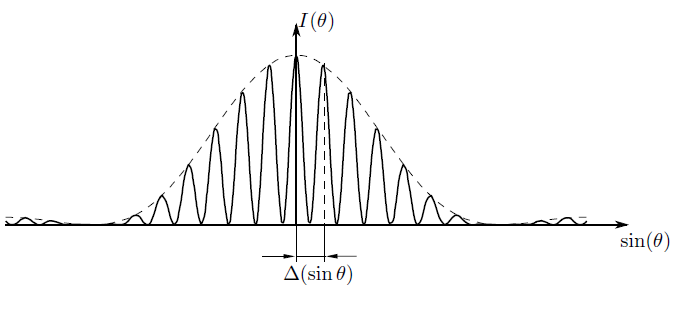
\includegraphics{fraun_two}
	\captionof{figure}{Дифракция Фраунгофера на двух щелях}
	
\end{center}
	\subparagraph{На решетке.}
	$$g_N(\theta) = g(\theta)\sum_{n= 0}^{N-1}\exp^{im\alpha}.$$
	$$|g_N(\theta)| = |g(\theta)|\cdot \left|\dfrac{\sin\frac{Nkd\sin\theta}{2}}{\sin\frac{kd\sin\theta}{2}}\right|.$$
	Характерной особенностью решётки является наличие узких максимумов, в которые идёт подавляющая доля общего потока энергии. Их
	положения определяются условием
	$$d\sin\theta_m = m\lambda$$
	\begin{center}
	
	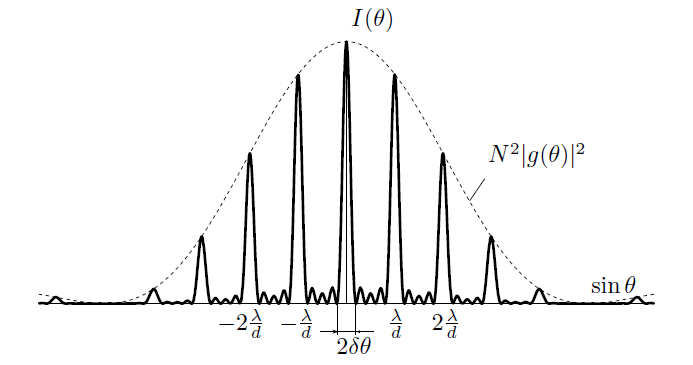
\includegraphics{fraun_resh}
	\captionof{figure}{Дифракция Фраунгофера на решетке}
	
\end{center}
	\subparagraph{На круглом отверстии.}
	При дифракции плоской волны на круглом отверстии в непрозрачном экране на удаленной плоскости наблюдения образуется картина дифракции: центральное яркое дифракционное пятно (пятно Эйри) окружено чередующимися светлыми и темными кольцами. Угловая полуширина пятна Эйри определяется условием $$\sin \theta = 1,22 \dfrac{\lambda }{D}$$
	
	\paragraph{Установки}
	\subparagraph{Дифракция Френеля на щели.}
	Схема установки для наблюдения дифракции Френеля представлена на рис. 1. Световые лучи освещают щель $S_2$ и испытывают на ней дифракцию. Дифракционная картина рассматривается с помощью микроскопа М, сфокусированного на некоторую плоскость наблюдения П.
	
	\begin{figure}[h]
		\centering
		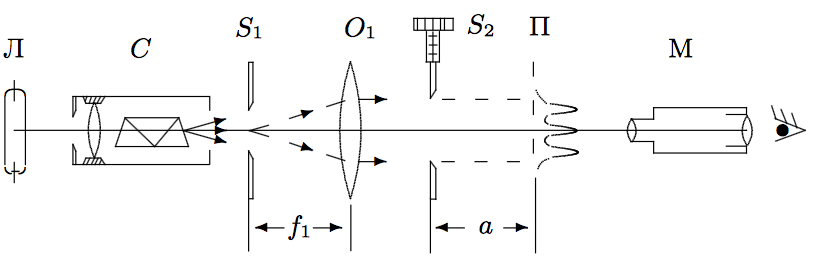
\includegraphics[width = \lw]{img1}
		\caption{Схема установки для наблюдения дифракции Френеля}
		\label{fig:scheme}
	\end{figure}
	
	
	Щель S2 освещается параллельным пучком монохроматического света с помощью коллиматора, образованного объективом $O_1$ и щелью $S_1$, находящейся в его фокусе. На щель $S_1$ сфокусировано изображение спектральной линии, выделенной из спектра ртутной лампы Л при помощи простого монохроматора C, в котором используется призма прямого зрения. 
	
	Распределение интенсивности света в плоскости наблюдения П проще всего рассчитывать с помощью зон Френеля (для щели их иногда называют зонами Шустера). При освещении щели $S_2$ параллельным пучком лучей (плоская волна) зоны Френеля представляют собой полоски, параллельные краям щели. Результирующая амплитуда в точке наблюдения определяется суперпозицией колебаний от тех зон Френеля, которые не перекрыты створками щели. Графическое определение результирующей амплитуды производится с помощью векторной диаграммы — спирали Корню. Суммарная ширина $n$ зон Френеля $\xi_n$ определяется соотношением: 
	\[ \xi_n = \sqrt{an\lambda}, \]
	
	где a~--~расстояние от щели до плоскости наблюдения (рис. \ref{fig:scheme}), а $\lambda$~--~длина волны.
	
	
	\subparagraph{Дифракция Фраунгофера на щели.}
	Картина дифракции резко упрощается, когда ширина щели становится значительно меньше ширины первой зоны Френеля. 
	
	Это условие всегда выполняется при достаточно большом расстоянии a от щели до плоскости наблюдения. Дифракционную картину, наблюдаемую в этом случае, принято называть дифракцией Фраунгофера. Исследование такой дифракционной картины заметно облегчается, потому что упрощаются фазовые соотношения.
	
	Дифракцию Френеля и Фраунгофера можно наблюдать на одной и той же установке (рис.~1). Однако при обычных размерах установки дифракция Фраунгофера возникает только при очень узких щелях. Например, при $a \approx 20-40cm$ и $\lambda \approx 5 \cdot 10^{-5}~cm$ получаем $D \ll 0.3~cm$. Поскольку работать с такими тонкими щелями неудобно, для наблюдения дифракции Фраунгофера к схеме, изображённой на рис. 1 добавляется объектив $O_2$ (рис.~\ref{img:fraung}).
	
	\begin{figure}[h]
		\centering
		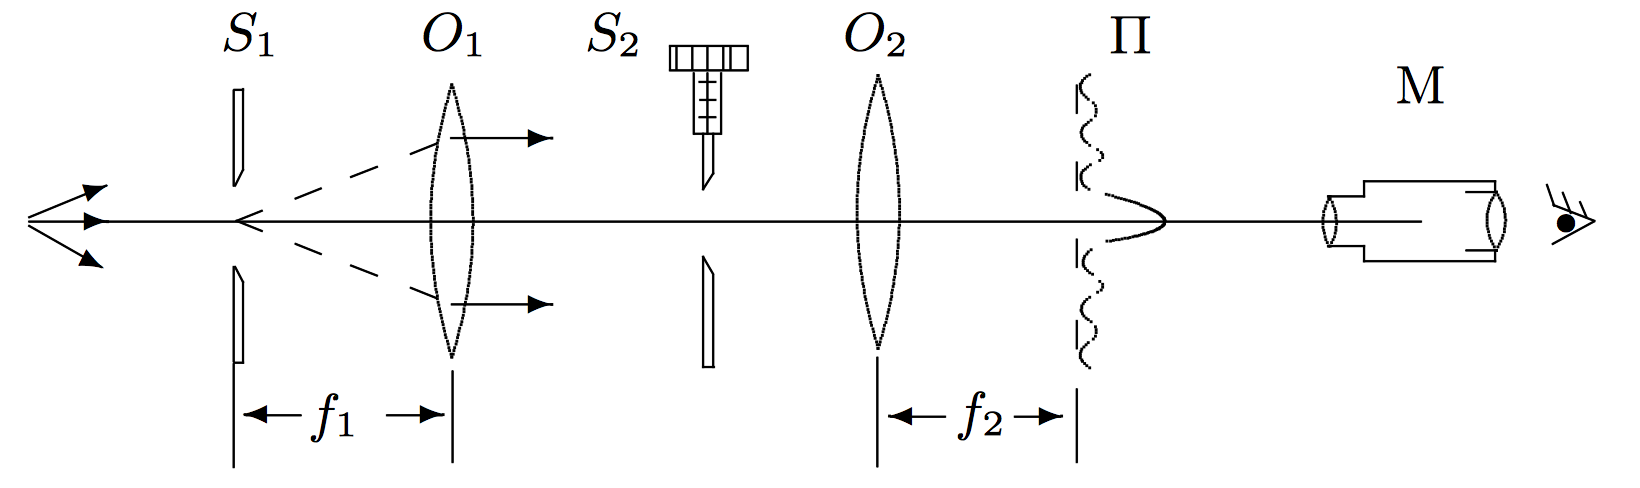
\includegraphics[width = 0.9 \lw]{img2}
		\caption{Схема установки для наблюдения дифракции Фраунгофера на щели}
		\label{img:fraung}
	\end{figure}
	
	Дифракционная картина наблюдается здесь в фокальной плоскости объектива $O_2$.
	
	
	\subparagraph{Дифракция Фраунгофера на двух щелях.}
	
	\begin{figure}[h]
		\centering
		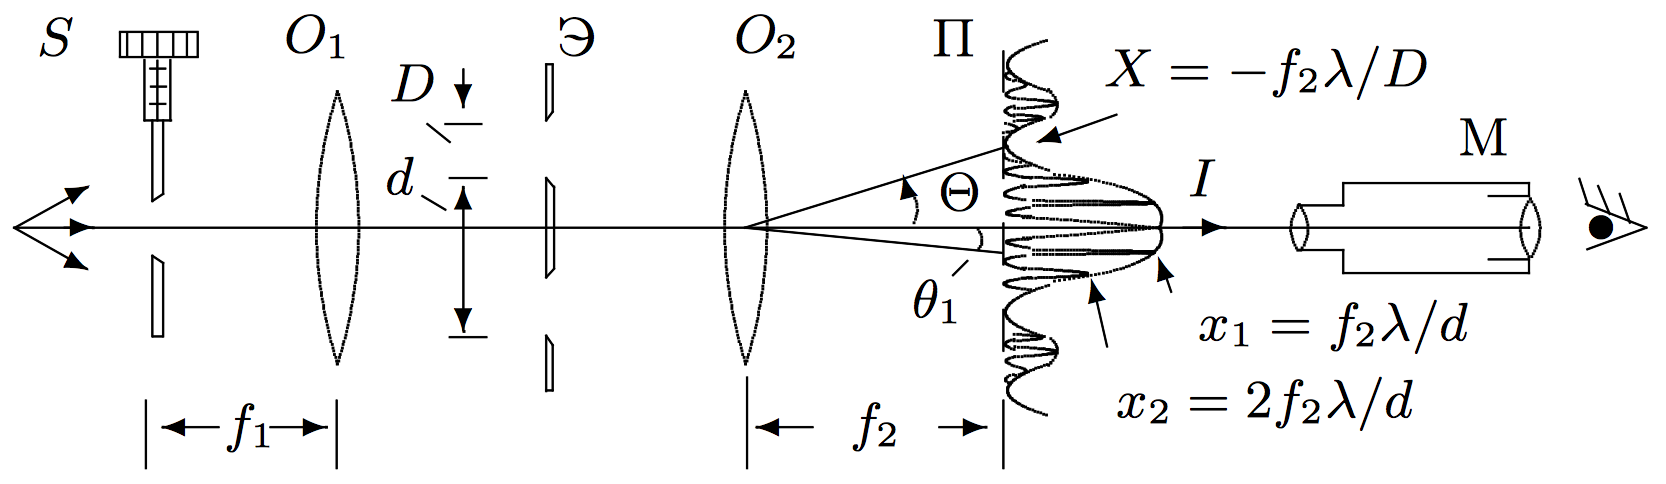
\includegraphics[width = 0.9 \lw]{img3}
		\caption{Схема установки для наблюдения дифракции Фраунгофера на двух щелях}
		\label{img:fraung_2}
	\end{figure}
	
	
	Для наблюдения дифракции Фраунгофера на двух щелях в установке (рис. \ref{img:fraung}) следует заменить щель $S_2$ экраном Э с двумя щелями (рис. \ref{img:fraung_2}). При этом для оценки влияния ширины входной щели на чёткость ди- фракционной картины вместо входной щели $S_1$ следует поставить щель с микрометрическим винтом. Два дифракционных изображения входной щели, одно из которых образовано лучами, прошедшими через левую, а другое — через правую щели, накладываются друг на друга.
	
	Если входная щель достаточно узка, то дифракционная картина в плоскости П (рис. \ref{img:fraung}) подобна той, что получалась при дифракции на одной щели (рис. \ref{img:fraung_2}), однако теперь вся картина испещрена рядом дополнительных узких полос. Наличие этих полос объясняется суперпозицией световых волн, приходящих в плоскость наблюдения через разные щели экрана Э.
	
	
	\subparagraph{Влияние дифракции на разрешающую способность оптического инструмента.}
	Установка, представленная на рис. \ref{img:dif}, позволяет исследовать влияние дифракции на разрешающую способность оптических инструментов.Как уже было выяснено, линзы $O_1$ и $O_2$ в отсутствие щели $S_2$ создают в плоскости П изображение щели $S_1$, и это изображение рассматривается в микроскоп М. Таким образом, нашу установку можно рассматривать как оптический инструмент, предназначенный для получения изображения предмета. При этом коллиматор (щель $S_1$ и объектив $O_1$) является моделью далёкого предмета, а объектив $O_2$ и микроскоп М составляют зрительную трубу, наведённую на этот предмет.
	Если перед объективом $O_2$ зрительной трубы расположить щель $S_2$, то изображение объекта будет искажено дифракцией на щели $S_2$. Чем меньше ширина $D_0$ этой щели, тем сильнее искажение. Качественной характеристикой этих искажений может служить минимальное угловое расстояние $\phi_{min}$ между объектами (источниками), которые ещё воспринимаются как раздельные.
	
	\begin{figure}[h]
		\centering
		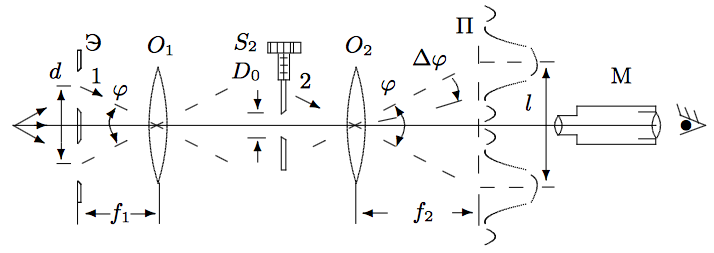
\includegraphics[width = 0.9 \lw]{img4}
		\caption{Схема установки для исследования разрешающей способности оптического инструмента}
		\label{img:dif}
	\end{figure}
	\end{document}